\documentclass[a4j]{celb-report}
%%%
%%% 計算機工学実験Bレポートテンプレート
%%%  このテンプレートを使う場合,celb-report.clsとjlisting.styが必要です.
%%%  このファイルと同じディレクトリに置いておいてください.
%%%

%%%
%%% まずはここで各種設定
%%%
\usepackage{comment}
\usepackage[dvipdfmx]{graphicx}
\period{3} % ← 何回目のレポートか(1~3)
\stunum{S123456} % ← 学生番号
\author{学生 なまえ} % ← 学生氏名
\date{1999年13月32日} % ← レポート提出日

\begin{document}

\maketitle

%%%%%%%%%%%%%%%%%%%%%%%%%%%%%%%%%%%%%%%%%%%%%%%%%%%%%%%%%%%%%%%%%%%%%
% レポート作成の手引:
%   レポート提出時は、ここから「レポート作成の手引ここまで」までの行をすべて削除すること!
%%%%%%%%%%%%%%%%%%%%%%%%%%%%%%%%%%%%%%%%%%%%%%%%%%%%%%%%%%%%%%%%%%%%%
\begin{comment}
\setcounter{section}{-1}
\section{レポート作成の手引}

各レポート,対応する回ごとに章(\verb|\section|)に分け,テキストの報告内容にて指示されている課題ごとに節(\verb|\subsection|)を用意して記載する.次章にて第1回分の例を記載しているので,適宜参考にすること.

% ----------------------------------------------------
\subsection{プログラムのソースコード,実行結果等を掲載する場合}

プログラムのソースコードや実行結果等を貼り付ける場合は,\verb|\lstlisting|環境を用いると良い.使い方は,このファイルの\texttt{tex}ソースを参考にすること.基本的には,ソースに記載の内容をコピーし,実行結果を書き換えると良い.
%
% --- 実行結果ここから
\begin{lstlisting}[basicstyle=\ttfamily\footnotesize, frame=single]

※※ ここに実行結果を貼り付ける. ※※
 
\end{lstlisting}
% --- 実行結果ここまで
%

% ----------------------------------------------------
\subsection{課題}

各回で用意されている考察・調査課題については,\verb|\kadai|を用いて,課題文と回答を記載する.第1回分の例を参考にすること.

% ----------------------------------------------------
\subsection{図の貼り付け}

図を貼り付ける場合は,\verb|\figure|環境を用いる.基本的には,このファイルの\texttt{tex}ソース内にある記述をそのまま用いれば良い.\verb|\includegraphcs|で画像ファイルを指定し,\verb|\caption|で図にキャプションを付ける.\verb|\label|は,本文中で図番号を参照するために付けておくラベルである(詳しくは後述).
%
\begin{figure}[htb]
 \centering 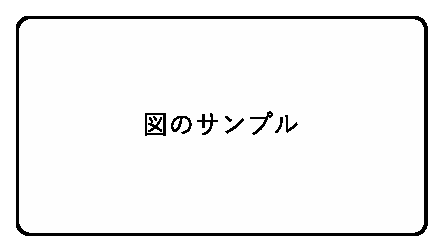
\includegraphics[scale=0.8]{sample-figure.eps}
 \caption{図のサンプル} \label{fig:sample}
\end{figure}
%

本文中で図を引用する場合は,図中で指定した\verb|label|を\verb|\ref|を用いて参照する.例えば上図で\verb|\label{fig:sample}|としている状態で本文中に``図\verb|\ref{fig:sample}|''と記述すると,texコンパイル後のファイルでは当該箇所が``図\ref{fig:sample}''に変換される.``図??''となる場合は,もう1度texコンパイルしてみて,それでも参照がされない場合は,ラベルが一致しているかどうか確認する.
% ----------------------------------------------------
\subsection{グループメンバーと役割分担}

%第3レポートの対象となる回では,複数人のグループで作業を行うため,各回で誰が何を担当したのかも節(\verb|\subsection|)を用いて記載する.以下は記載例である.\texttt{tex}ソースに記載の通り,\verb|\description|環境を用いると良い.
%
\begin{description}
 \item[s123456 学生 なまえ] ネットワークの配線,環境の構築
 \item[s135791 相方 ひとりめ] プログラムのコーディング,デバッグ
 \item[s246802 相方 ふたりめ] コーディングのサポート
 \item[s369258 相方 さんにんめ] 3人の応援
\end{description}

% ----------------------------------------------------
%\subsection{参考文献等}

%書籍,インターネット上の情報などを参考にした場合,対象となるすべての回のものをまとめて,\verb|\thebibliography|環境を用いて出展を明記する.書き方は本ファイルの\texttt{tex}ソースを参考にする.
%
%%%%%%%%%%%%%%%%%%%%%%%%%%%%%%%%%%%%%%%%%%%%%%%%%%%%%%%%%%%%%%%%%%%%%
% レポート作成の手引ここまで
%%%%%%%%%%%%%%%%%%%%%%%%%%%%%%%%%%%%%%%%%%%%%%%%%%%%%%%%%%%%%%%%%%%%%


%%%%%%%%%%%%%%%%%%%%%%%%%%%%%%%%%%%%%%%%%%%%%%%%%%%%%%%%%%%%%%%%%%%%%
% 第1回分(第1レポート内)サンプル
%   第1レポートでは,第1回~第4回分それぞれを 章 (\section) として1つのレポートにまとめること
%%%%%%%%%%%%%%%%%%%%%%%%%%%%%%%%%%%%%%%%%%%%%%%%%%%%%%%%%%%%%%%%%%%%%
%%% ------------------------------------------------------------------
\newpage % ← 改ページ
\section{第1回 誤り制御符号(1):パリティ符号}

% ----------------------------------------------------
\subsection{実行結果}

%
% --- 実行結果ここから
\begin{lstlisting}[basicstyle=\ttfamily\footnotesize, frame=single]
$ ./parity



...


 
\end{lstlisting}
% --- 実行結果ここまで
%

\subsection{実行結果に対する考察}
前節の実行結果より,~であることがわかる.また,~であるものと考えられる.


% ----------------------------------------------------
\subsection{課題}

\kadai{今回の実験で作成したパリティ符号は,偶数パリティと奇数パリティのいずれであるかを答えよ.}

~~~であるため,◯数パリティである.

\kadai{1ビット水平パリティ符号について調査せよ.}

1ビット水平パリティ符号とは,~~ものである.~~.

\kadai{1ビット水平パリティ符号と1ビット垂直パリティ符号を組み合わせることにより,1ビットの誤りを訂正できることを示せ.}

~~.

以上より,1ビット水平パリティ符号と~~~,~~~できる.
\end{comment}
%
%%%%%%%%%%%%%%%%%%%%%%%%%%%%%%%%%%%%%%%%%%%%%%%%%%%%%%%%%%%%%%%%%%%%%
% 第1回分サンプルここまで
%%%%%%%%%%%%%%%%%%%%%%%%%%%%%%%%%%%%%%%%%%%%%%%%%%%%%%%%%%%%%%%%%%%%%

%%% ------------------------------------------------------------------
\section{第9回 無線LAN(1):通信の基礎}
\subsection{グループメンバーと役割分担}
%第3レポートの対象となる回では,複数人のグループで作業を行うため,各回で誰が何を担当したのかも節(\verb|\subsection|)を用いて記載する.以下は記載例である.\texttt{tex}ソースに記載の通り,\verb|\description|環境を用いると良い.
%
\begin{description}
 \item[s123456 学生 なまえ] ネットワークの配線,環境の構築
 \item[s135791 相方 ひとりめ] プログラムのコーディング,デバッグ
 \item[s246802 相方 ふたりめ] コーディングのサポート
 \item[s369258 相方 さんにんめ] 3人の応援
\end{description}
%\subsection{解析対象側の情報(解析対象側のネットワークを構築した場合のみ)}
%解析対象側のネットワークにおいて, AP に設定されていた ESSID ,および ECHO クライアントに入力した文字列を記載する.
\setcounter{subsection}{2}
\subsection{解析対象APの情報}
%解析対象側のネットワークにおいて, AP に設定されていた ESSID ,および ECHO クライアントに入力した文字列を記載する.
解析の結果、以下のような情報が得られた。
\lstinputlisting[caption=解析対象の情報1]{../LAN1/sysExp1/text.txt}
\lstinputlisting[caption=解析対象の情報2]{../LAN1/sysExp2/text.txt}
\lstinputlisting[caption=解析対象の情報3]{../LAN1/sysExp3/text.txt}
\subsection{解析結果}
%解析した TCP パケットの内容(詳細ペイン,バイトペインの内容:それぞれテキストとして抽出する)と,そこから得られた ECHO サーバ/クライアント間における通信内容(交換している文字列)を記載する.
\begin{center}
 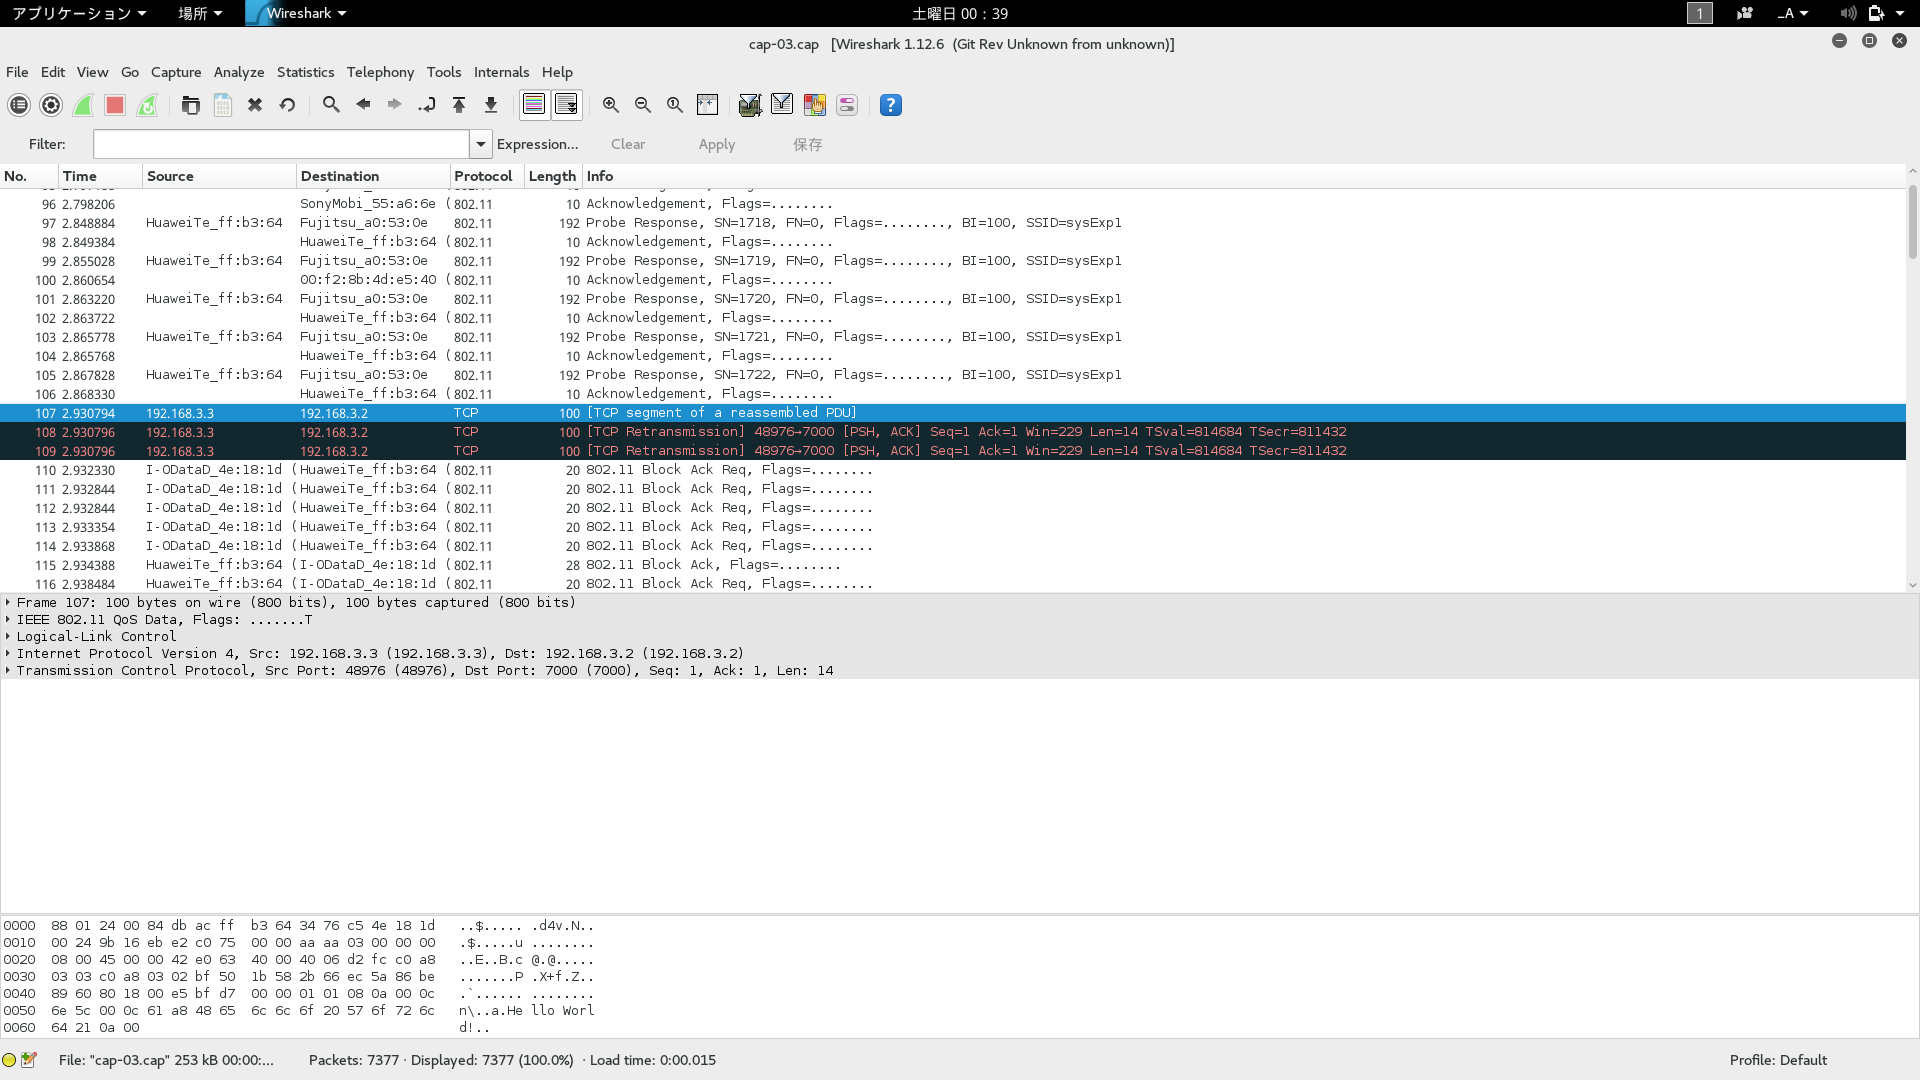
\includegraphics[width=17cm]{../LAN1/sysExp1/Screenshot.png}
\end{center}
上の画像の通りHello World!という文字列が得られた。
\begin{center}
 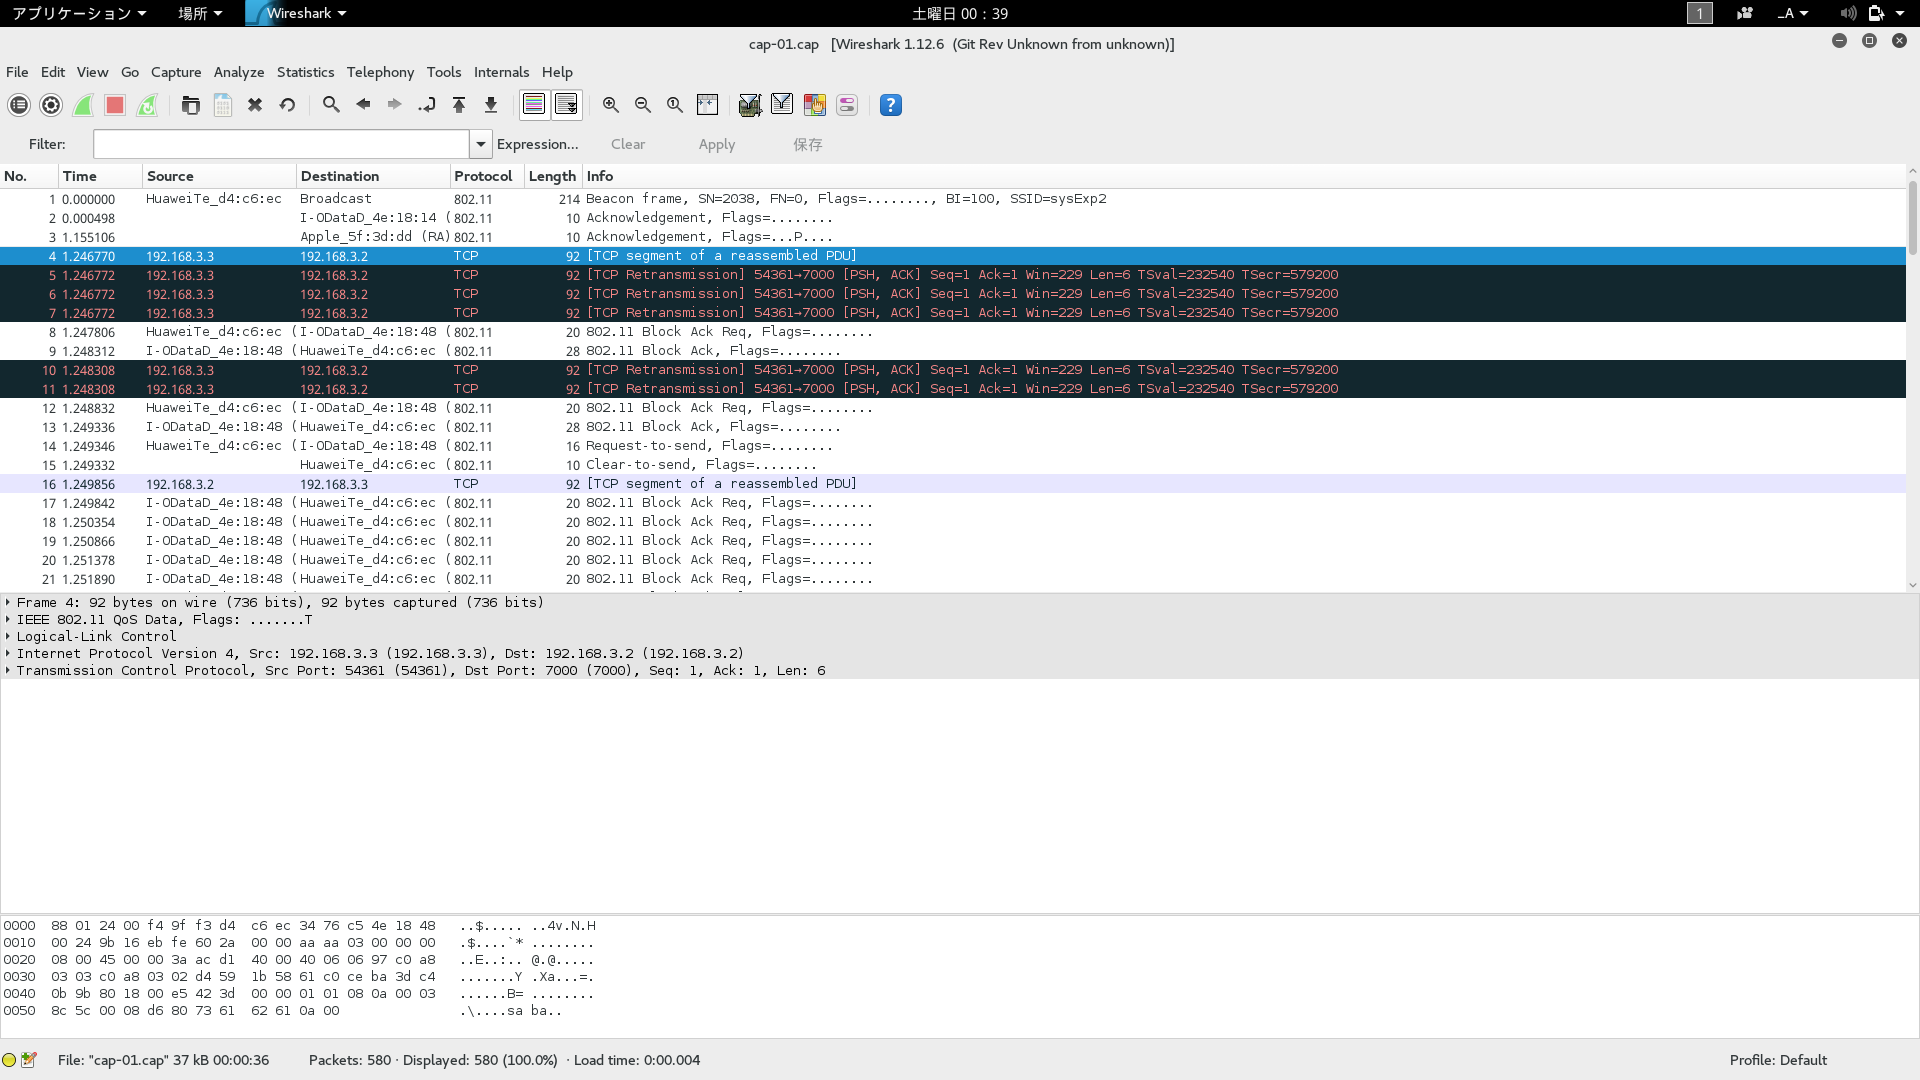
\includegraphics[width=17cm]{../LAN1/sysExp2/Screenshot.png}
\end{center}
上の画像の通りsabaという文字列が得られた。
\begin{center}
 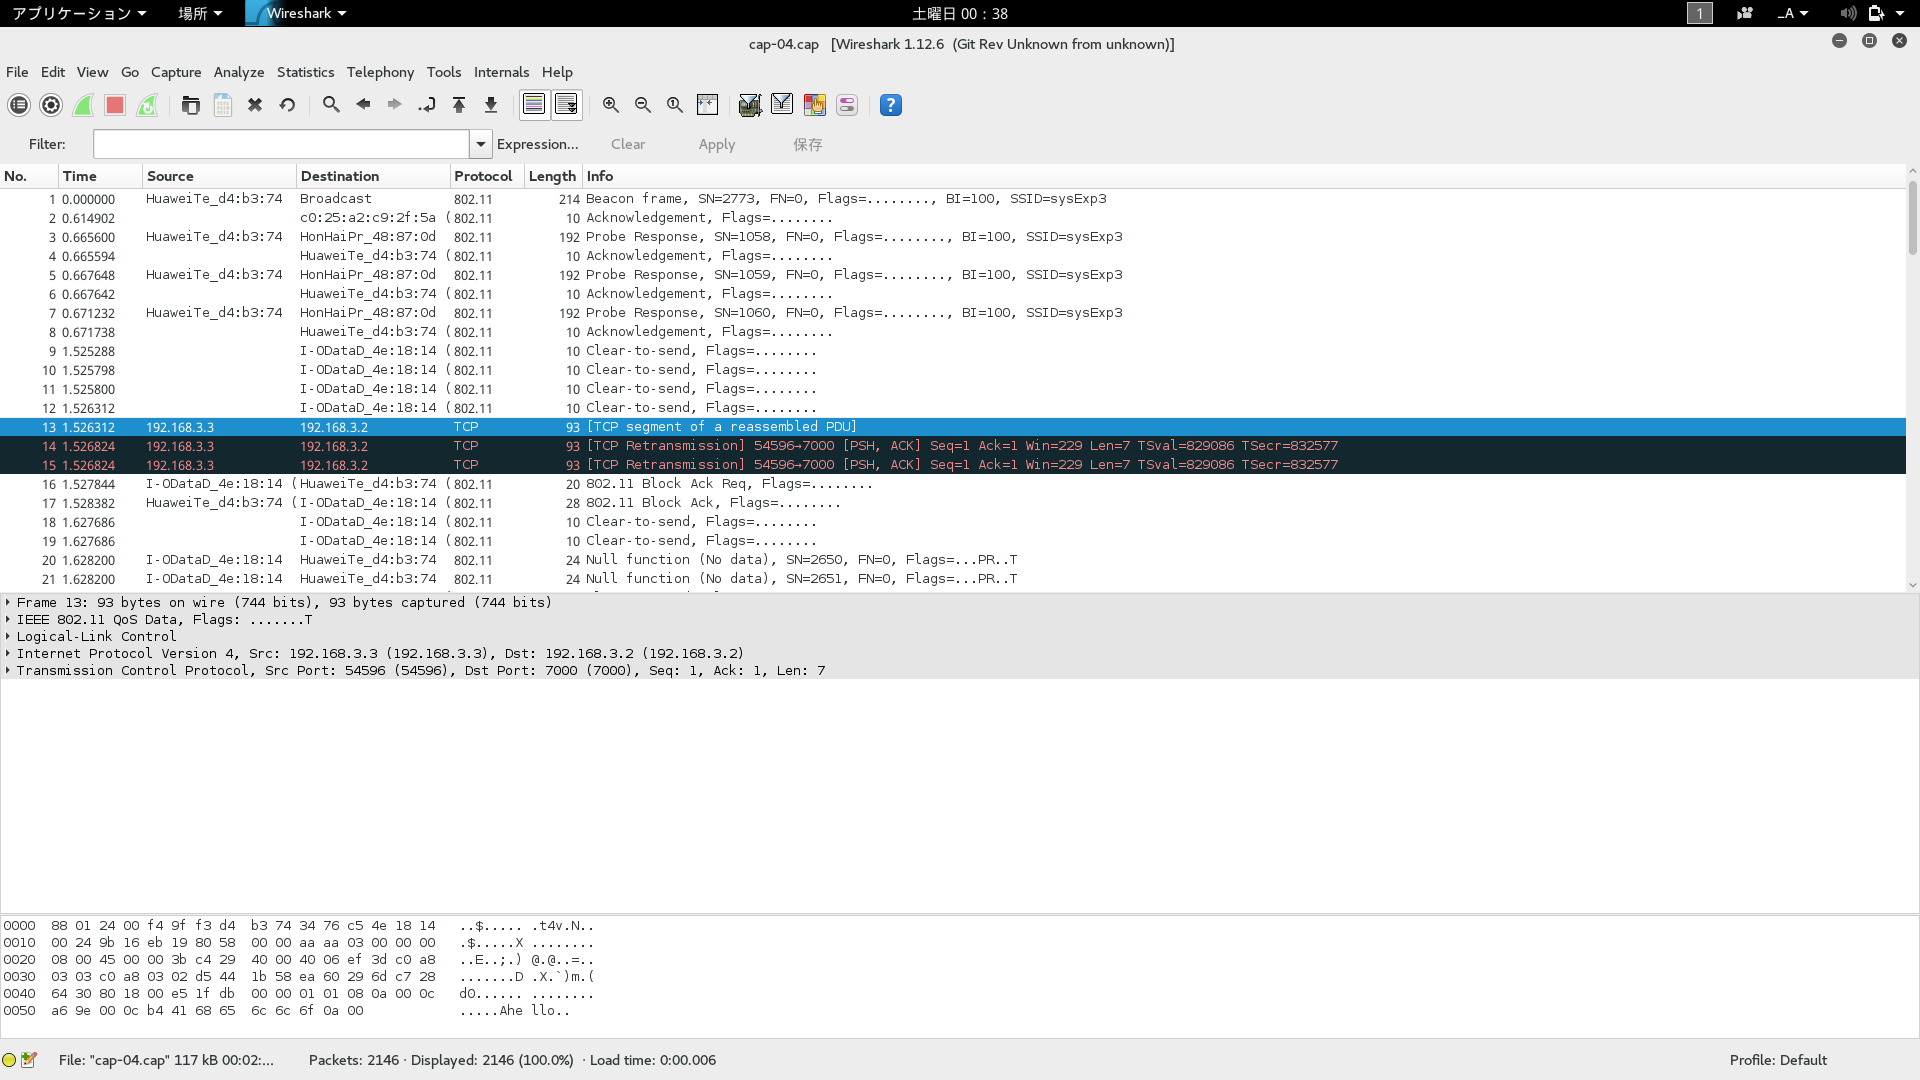
\includegraphics[width=17cm]{../LAN1/sysExp3/Screenshot.png}
\end{center}
上の画像の通りhelloという文字列が得られた。
\subsection{調査課題}
%次に示す課題について調査・検討し,レポートにて報告せよ.インターネット上の情報を参考にするときは,出典( URLなど)を記載すること.コピー&ペーストではなく,自分なりにまとめる形にすること.
\begin{enumerate}
\renewcommand{\labelenumi}{(\arabic{enumi})}
 \item Wireshark による解析結果には, TCP パケットだけでなく,無線 LAN 特有の制御フレームも表示される.この中で交換されている Request-to-Send (RTS) および Clear-to-Send (CTS) について調査し,これらを用いた通信開始手順について説明せよ.\\
\\
RTSとCTSは複数の端末が同時にデータを送信しようとして起こる衝突を防ぐための仕組みで、データを送信しようとする端末はいきなりデータをアクセスポイントに送るのではなく、まずアクセスポイントに対してデータを送信するための許可をもらう。これをRTSという。そしてRTSを受けたアクセスポイントがデータを送信する許可を出す。これをCTSという。\\
 \item 無線 LAN における MAC プロトコルである CSMA/CA では,通信の衝突を避けるための機構としてバックオフと呼ばれる手法を用いている.このバックオフについて調査し,動作を説明せよ.\\
\\
データの送信で衝突が起きた時、ランダムな時間待ってから再送する制御をバックオフという。
\end{enumerate}

% ----------------------------------------------------

%%% ------------------------------------------------------------------
\newpage
\section{第10回 無線LAN(2):通信の暗号化}
\subsection{グループメンバーと役割分担}
%第3レポートの対象となる回では,複数人のグループで作業を行うため,各回で誰が何を担当したのかも節(\verb|\subsection|)を用いて記載する.以下は記載例である.\texttt{tex}ソースに記載の通り,\verb|\description|環境を用いると良い.
%
\begin{description}
 \item[s123456 学生 なまえ] ネットワークの配線,環境の構築
 \item[s135791 相方 ひとりめ] プログラムのコーディング,デバッグ
 \item[s246802 相方 ふたりめ] コーディングのサポート
 \item[s369258 相方 さんにんめ] 3人の応援
\end{description}
%\subsection{解析対象側の情報(解析対象側のネットワークを構築した場合のみ)}
%解析対象側のネットワークにおいて, AP に設定されていた ESSID ,および ECHO クライアントに入力した文字列を記載する.
\setcounter{subsection}{2}
\subsection{解析対象APの情報}
解析対象とした AP の ESSID および BSSID を記載する.
\lstinputlisting[caption=解析対象のAP]{../LAN2/AP.txt}
%\subsection{ARP リプレイ攻撃の実行結果(実行した場合のみ)}
%5.4節(付録B)の各コマンドを実行した際の出力結果を掲載する.実行結果が行数が多い場合には,適当に途中を省略しても良い.
\subsection{解析結果}
5.5節において,aircrack-ngによってWEPキーが解析できた際の出力結果を掲載する.5.3節におけるairodump-ng実行時の出力結果は不要である.
また,前回の実験と同様,Wiresharkで解析したTCPパケットの内容(詳細ペイン,バイトペインの内容:それぞれスクリーンショットを貼り付ける)と,そこから得られたECHOサーバ/クライアント間における通信内容(交換している文字列)を記載する.
\lstinputlisting[caption=解析結果]{../LAN2/text.txt}
\begin{center}
 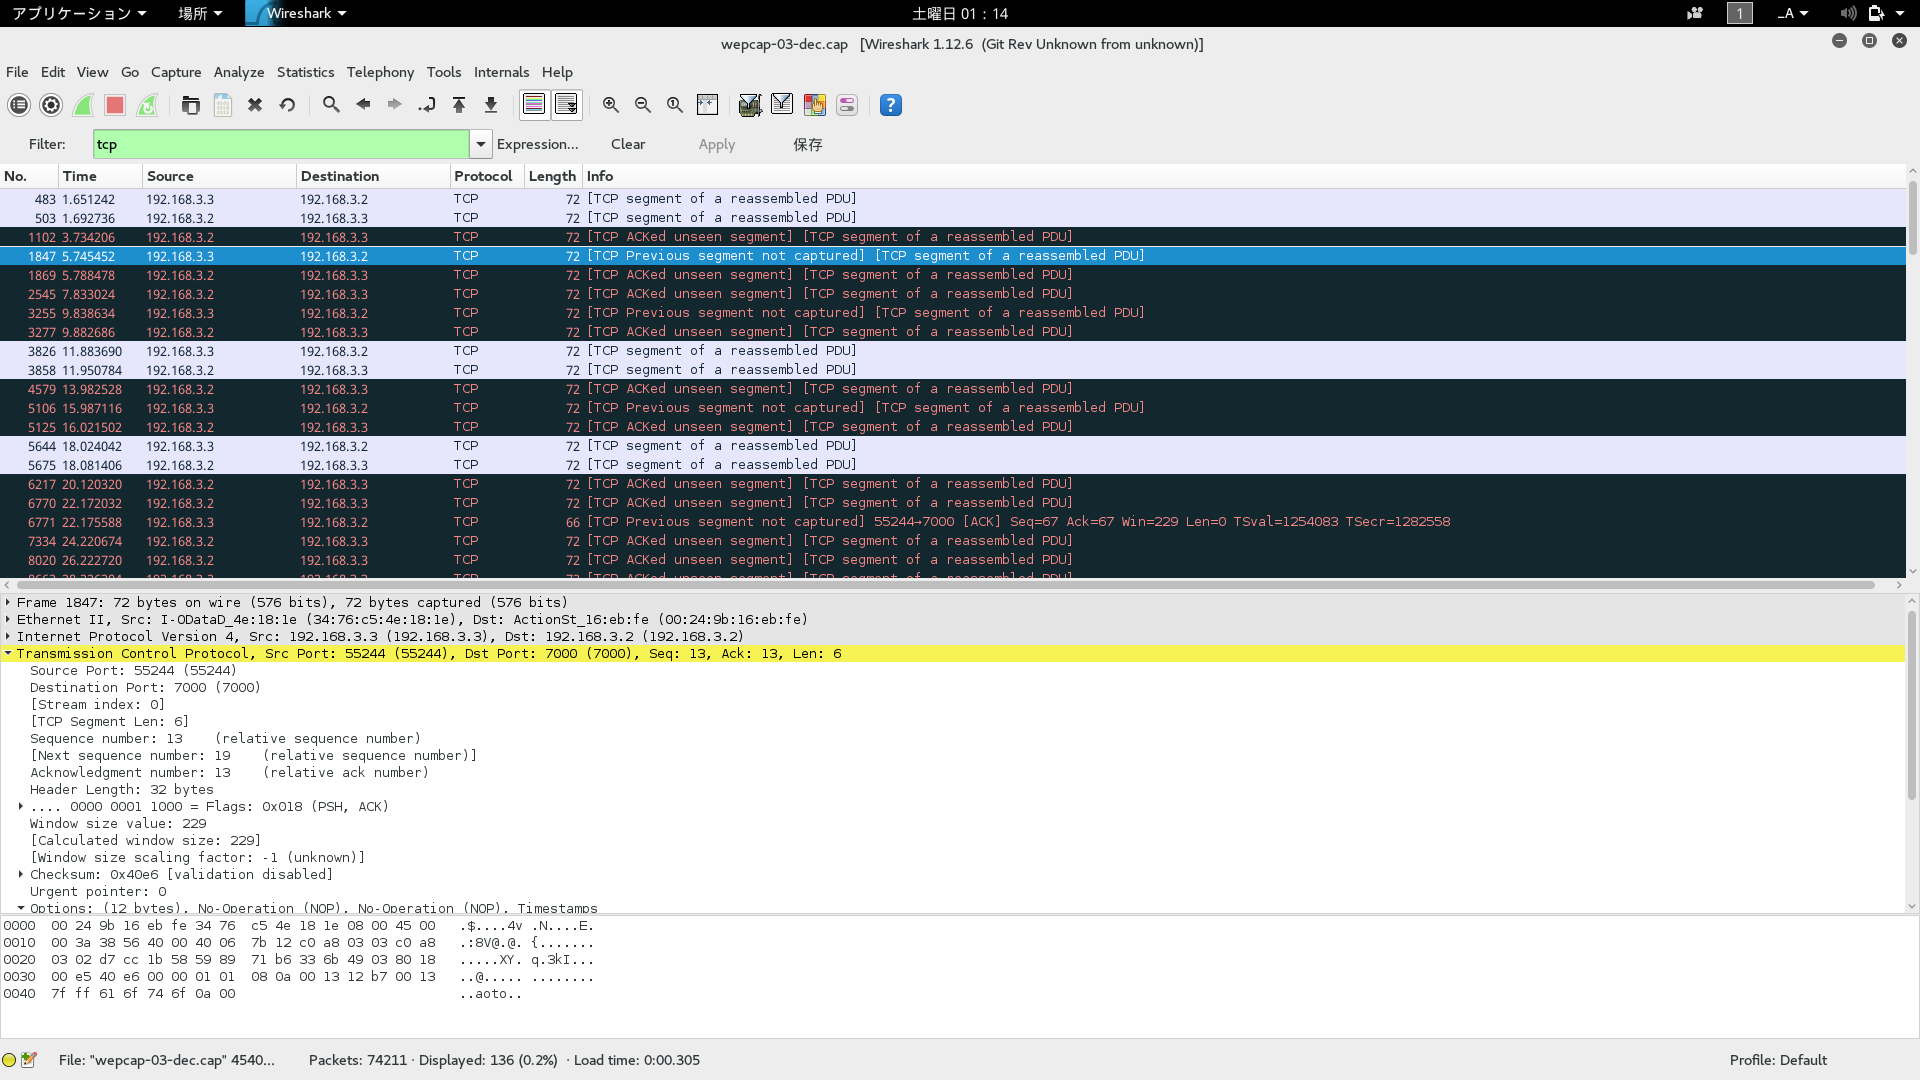
\includegraphics[width=17cm]{../LAN2/screenshot.png}
\end{center}
\subsection{調査課題}
次に示す課題について調査・検討し,レポートにて報告せよ.インターネット上の情報を参考にするときは,出典(URLなど)を記載すること.コピー\&ペーストではなく,自分なりにまとめる形にすること.
\begin{enumerate}
 \renewcommand{\labelenumi}{(\arabic{enumi})}
 \item 今回の攻撃で用いたARPについて調査し,何を行うためのプロトコルであり,どのような情報がやり取りされるか,簡潔に説明せよ.\\
\quad ARP(Address Resolution Protocol)は通信相手のIPアドレスからEthernetのMACアドレスを得るプロトコルで、ある端末がTCP/IPで別の端末と通信しようとするとき、通信相手の端末のIPアドレスからMACアドレスを得るためにネットワーク内の全ノードにARPリクエストを送る。ARPリクエストには通信相手のIPアドレスが含まれていて、ARPリクエストを受信した端末はARPリクエストのIPアドレスと自分のIPアドレスが等しい場合、自分のMACアドレスをARPリプライとして送信し、ARPリクエストを送信した端末がMACアドレスを得る。
 \item 無線LANのセキュリティとして,暗号化以外に用いられているものについて,どのようなものがあるか調査し,簡潔に説明せよ.\\
\quad 暗号化以外の無線LANのセキュリティとして、接続制限が挙げられる。アクセスポイントが通信しようとする端末のMACアドレスなどの情報を取り、特定の端末のみに通信の許可を出したり、特定の端末との通信を禁止したりして接続を制限する方法である。
\end{enumerate}
%%% ------------------------------------------------------------------
% --- 参考文献リストここから
\newpage
\begin{thebibliography}{9}
%\bibitem{book-sample} 神崎映光,西川津ビビッド,出雲島猫,「書籍の参照はこんな感じ」,島大出版,1979年.
%\bibitem{url-sample} 島根大学 総合理工学部 数理・情報システム学科(情報系),http://www.cis.shimane-u.ac.jp/.
\bibitem{RTSandCTS} Wireless LAN - CSMA/CA , http://www.infraexpert.com/study/wireless6.html
\bibitem{Backoff} 第6回 イーサネット(その1) - イーサネットの規格とCSMA/CDアクセス制御方式 (4/5) , http://www.atmarkit.co.jp/ait/articles/0105/23/news004\_4.html
\bibitem{ARP} TCP/IP - ARP , http://www.infraexpert.com/study/tcpip2.html
\end{thebibliography}
% --- 参考文献リストここまで
%

\end{document}
